\subsection{Сумерки}
\term{Сумерки}~--- часть суток, когда Солнце находится неглубоко под горизонтом. 

Различают сумерки \imp{гражданские}, \imp{навигационные} и \imp{астрономические}. 

Высота Солнца в зависимости от вида сумерек:
\begin{enumerate}
\item Гражданские~--- от $0^{\circ}$ до $-6^{\circ}$
\item Навигационные~--- от $-6^{\circ}$ до $-12^{\circ}$
\item Астрономические~--- от $-12^{\circ}$ до $-18^{\circ}$
\end{enumerate}

Когда Солнце опускается ниже $-18^{\circ}$, наступает ночь.

\begin{center}
\begin{figure}[h!]
\centering
 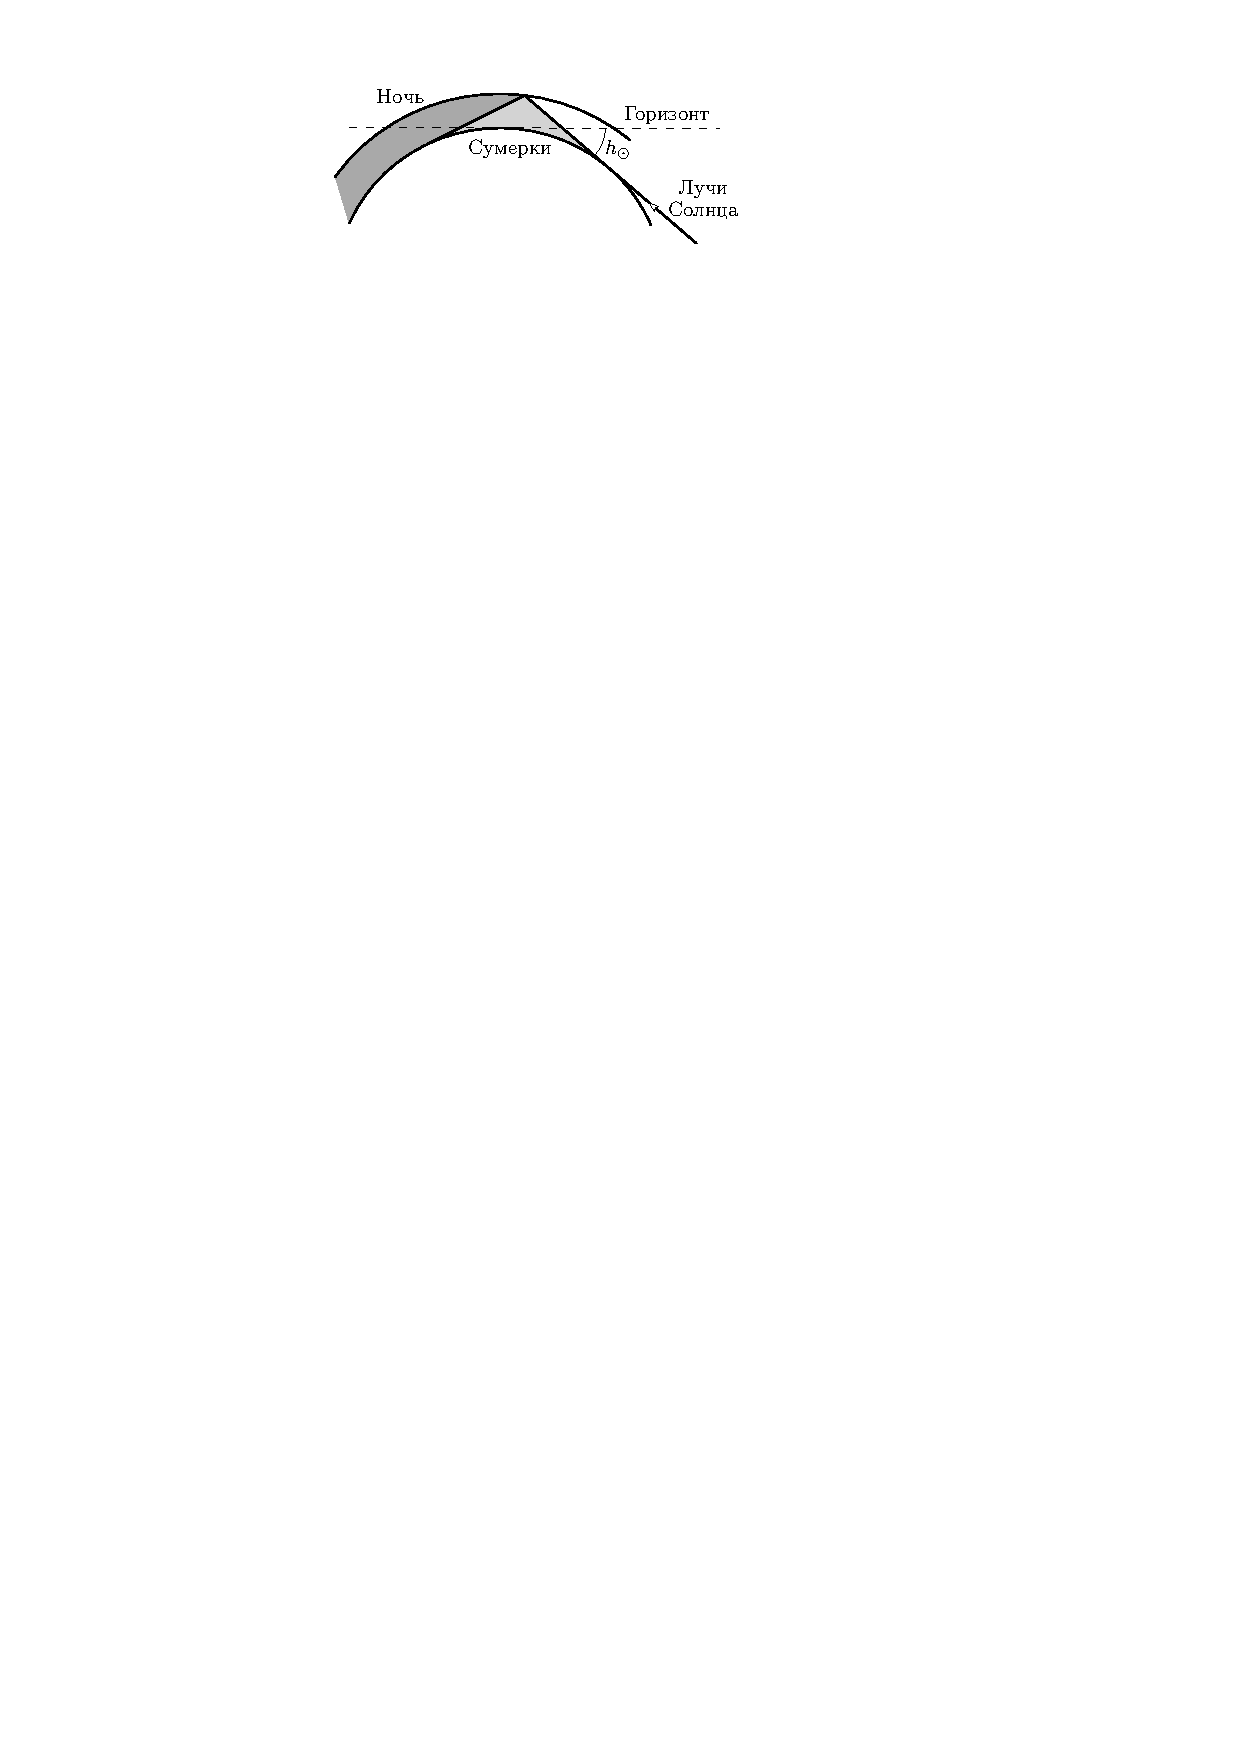
\includegraphics[width=0.65\textwidth]{spher-astro-dusk.pdf}
 \caption{Сумерки}
\end{figure}
\end{center}